\chapter{Implementácia FPGA MITM obvodu}
\label{kap:implementacia}

V tejto kapitole navrhneme a implementujeme hardvérový MITM obvodu pomocou FPGA. Hlavným cieľom bude možnosť podpory pre viacero zbernicových protokolov. A snaha o abstrakciu detailov fyzického protokolu zbernice pred samotnou MITM logikou obvodu. Ako sme v časti \ref{sek:masterSlave} spomenuli, niektoré vlastnosti principiálne nemožno abstrahovať. Napriek tomu ukážeme, že viacero vlastností možno pred vyššou vrstvou zakryť. Tento prístup zároveň umožní pomerne jednoduché rozšírenie o podporu ďalších zbernicových protokolov. V práci sa zameriame na konkrétne dva -- UART a SPI. Dôvodom výberu týchto dvoch zberníc je fakt, že princíp ich fungovania je značne odlišný ako sme detailnejšie uviedli v kapitole \ref{kap:zbernice}.

\section{Technické aspekty implementácie}
V tejto časti opíšeme po technickej stránke spôsob, ktorým sme sa rozhodli implementovať hardvérový MITM obvod. Obvod implementujeme pomocou FPGA technológie, ktorá umožňuje obvod flexibilne nakonfigurovať a upravovať podľa potreby. Výhodou oproti štandardnému softvérovému prístupu s využitím všeobecne určeného (angl. general purpose) procesora je možnosť kontroly nad spracovaním informácie na úrovni logických hradiel. To umožňuje jednoduchšiu a najmä rýchlejšiu manipuláciu s fyzickou vrstvou signálov na zberniciach a ich spracovanie.

\subsection{Hardvér}
Čo sa týka hardvéru, v práci sme sa rozhodli pracovať s dvoma FPGA vývojovými doskamiod spoločnosti Lattice Semiconductor, konkrétne dosky iCEstick Evaluation Kit, ďalej len icestick a iCE40-HX8K Breakout Board, ďalej len doska HX8K. Na obrázku \ref{obr:iceHw} možno vidieť pohľad z vrchu na obidve dosky. Obidve dosky obsahujú čipy zo sady iCE40-HX. Vývojová doska icestick obsahuje lacnejší FPGA čip iCE40-HX1K, ktorý obsahuje pomerne málo logických buniek pre skladanie FPGA obvodu. Pre komplikovanejšie obvody, ktorých konfigurácia sa na tento FPGA čip nemusí zmestiť preto použijeme dosku HX8K, ktorá obsahuje čip iCE40-HX8K. Ten má približne osemkrát viac logických buniek, čo pre naše účely postačuje. Dôvodom výberu týchto vývojových dosiek je priamočiara podpora open source softvérových nástrojov pre syntézu FPGA kódu. Ďalej dosky obsahujú prevodník z USB na UART, ktorý umožňuje jednoduché nahranie výslednej konfigurácie obvodu na FPGA čip.

\begin{figure}
    \centering
    \subfloat[Icestick Evaluation Kit]{\includegraphics[width=0.6\textwidth]{images/icestickHw.png}}
    \hfill
    \subfloat[iCE40-HX8K Breakout Board]{\includegraphics[width=0.4\textwidth]{images/hx8kBoardHw.png}}
    \caption[Vývojové dosky FPGA iCE40]{Vývojové dosky FPGA iCE40. Zdroj: https://www.latticesemi.com}
    \label{obr:iceHw}
\end{figure}

\subsection{Jazyk Verilog}
Existuje viacero jazykov pre popisovanie hardvéru, najrozšírenejšími sú VHDL a Verilog. MITM obvod sme sa rozhodli implementovať v jazyku Verilog. Dôvodom bola podpora jazyka open source nástrojmi, ktoré popíšeme v ďalšej časti. V nasledujúcich častiach podrobnejšie popíšeme spôsob implementácie nášho MITM obvodu. V týchto častiach predpokladáme, že čitateľ pozná syntax a základné princípy písania kódu v jazyku Verilog.

\subsection{Softvérové nástroje}\label{sek:software}
Pre účely syntézy, testovania a simulácie kódu, sme využili viacero softvérových nástrojov. Všetky použité nástroje sú open source a sú zadarmo dostupné. V tejto časti jednotlivé nástroje stručne opíšeme:

\textbf{Yosys} (Yosys Open SYnthesis Suite) \cite{yosys} je hlavný nástroj, ktorý sme použili pre syntézu Verilog kódu. Jeho výstupom je tzv. netlist, ktorý reprezentuje výslednú FPGA konfiguráciu, presnejšie logické prepojenie jednotlivých komponentov na FPGA (logické bunky, pamäťové členy, vstupno-výstupné porty a pod.).

\textbf{NextPNR} (Next Place and Route) \cite{nextpnr} je ďalším nástrojom v reťazi, ktorého vstupom je netlist vygenerovaný predchádzajúcim nástrojom yosys. Tento nástroj má za úlohu naplánovať fyzické rozmiestnenie jednotlivých hardvérových komponentov a ich prepojenie pomocou vodičov. Pri tomto kroku je špeciálne dôležité naplánovať obvod tak, aby boli pri propagácií signálu medzi fyzickými časťami obvodu dodržané časové obmedzenia (angl. timing constraints). Výstup sa zvykne nazývať plánovaný (routed) netlist.

\textbf{Project IceStorm} \cite{icestorm} je sada nástrojov, pre prácu s FPGA obvodmi z rodiny iCE40, ktorý bol vyvinutý pomocou reverzného inžinierstva. V práci sme použili nasledovné nástroje z projektu IceStorm:\\
\textbf{icepack} -- posledný nástroj v \uv{kompilačnej} reťazi. Vstupom je plánovaný netlist vygenerovaný pomocou nextPNR. Tento vstup zakóduje do tzv. bitstreamu, čo je binárny formát, ktorý možno priamo nahrať na samotnú FPGA dosku.\\
\textbf{iceprog} -- nástroj, ktorý umožňuje nahrať výsledný bitstream na FPGA dosku.\\
\textbf{icetime} -- pomocný nástroj, ktorý overí dodržanie časové obmedzení. Vstupom je plánovaný netlist a výstupom je textová správa popisujúca výsledok overovania.\\
\textbf{icepll} -- pomocný nástroj, ktorý na základe vstupnej a požadovanej výstupnej frekvencie vypočíta potrebné parametre pre nastavenie PLL obvodu pre generovanie hodinového signálu. Výsledné parametre možno potom použiť priamo vo Verilog kóde pri inštanciácií PLL modulu.

\textbf{ICARUS Verilog} \cite{iverilog} je ďalším nástrojom, ktorý sme pri implementácií použili. Tento nástroj je podobne ako yosys syntetizátor Verilog kódu, jeho účelom nie je však generovanie fyzicky použiteľnej FPGA konfigurácie, ale simulácia FPGA obvodu. Výstupom je VVP (Verilog VPI Processor) kód, ktorý možno simulovať napríklad pomocou nástroja \textbf{vvp} (súčasťou projektu ICARUS Verilog). Výsledkom simulácie je súbor simulačných dát, napríklad vo VCD formáte.

\textbf{GTKWave} \cite{gtkwave} je nástroj, ktorý dokáže vizuálne reprezentovať priebeh signálov zo simulačných dát. Tento nástroj sme spolu s nástrojom ICARUS Verilog použili na testovanie a odhalenie logických chýb pri implementácii FPGA obvodu.

V nasledujúcich častiach detailnejšie opíšeme našu implementáciu jednotlivých častí FPGA obvodu.

\section{Hlavný modul obvodu}
Celý obvod sa na najvyššej úrovni bude skladať z hlavného modulu (Top Level Module), ktorý zastrešuje celý obvod a obsahuje vstupy a výstupy, ktoré budú pripojené k fyzickým I/O portom. Všetky externé vstupy je potrebné synchronizovať. Synchronizácia zabezpečí, že všetky hrany (zmeny signálu z 0 na 1, resp. naopak) výsledného signálu budu synchrónne s globálnymi systémovými hodinami. Spôsob implementácie synchronizačného obvodu bližšie popíšeme v časti \ref{subsek:synchronizer}.

\subsection{Systémové hodiny}
Systémový hodinový signál, ďalej len systémové hodiny, je generovaný pomocou PLL obvodu. Využijeme PLL obvod, ktorý nám poskytuje knižnica pre prácu s iCE40 FPGA čipmi, podporovaná aj nami zvoleným yosys syntetizátorom. Ako referenčný vstup pre PLL obvod pripojíme 12\,MHz oscilátor, ktorý sa nachádza na obidvoch doskách icestick, resp. HX8K. Tento vstup, narozdiel od ostatných, nie je potrebné synchronizovať. Výstupnú frekvenciu PLL obvodu ponecháme ako voliteľný parameter, pričom podporované frekvencie sú z rozsahu 16 -- 275\,MHz.

Pre tento účel použijeme nástroj icepll spomenutý v časti \ref{sek:software}, ktorý zo vstupnej a požadovanej výstupnej frekvencie dokáže vygenerovať priamo Verilog kód, ktorý inštancuje knižničný modul s potrebnými parametrami.
Tento proces využijeme pri automatizovanej syntéze kódu pomocou nástroja GNU make. Nie všetky hodnoty z rozsahu je možné dosiahnuť, v prípade, že požadovaná výstupná frekvencia nie je možná, nástroj vygeneruje kód, ktorý nakonfiguruje najbližšiu možnú frekvenciu k požadovanej.

\subsection{Ostatné časti obvodu}
Okrem generovania systémových hodín a synchronizácie vstupu bude hlavný modul pozostávať z troch dôležitých pod-modulov, ktorých implementáciu bližšie popíšeme v príslušných častiach. Prvým pod-modulom je rozhranie, ktoré zakrýva detaily zbernice (Bus Interface) a sú k nemu pripojené vstupy a výstupy zbernicových liniek oboch strán. I/O Hadler je modul pre spracovanie ostatných vstupov a výstupov netýkajúcich sa priamo zbernice, napr. globálny reset signál, LED indikujúca prebiehajúcu komunikáciu, žiadosť o zmenu režimu MITM logiky a pod. Posledným a najdôležitejším modulom je MITM logika, ktorú treba naprogramovať podľa konkrétneho útoku s využitím zbernicového rozhrania. Pri návrhu obvodu pre MITM logiku možno využiť vybrané vstupy z modulu I/O handler, pre dynamické nastavenie logiky. Schéma hlavného modulu je na obrázku \ref{obr:topLevelModule}.

\begin{figure}
    \centerline{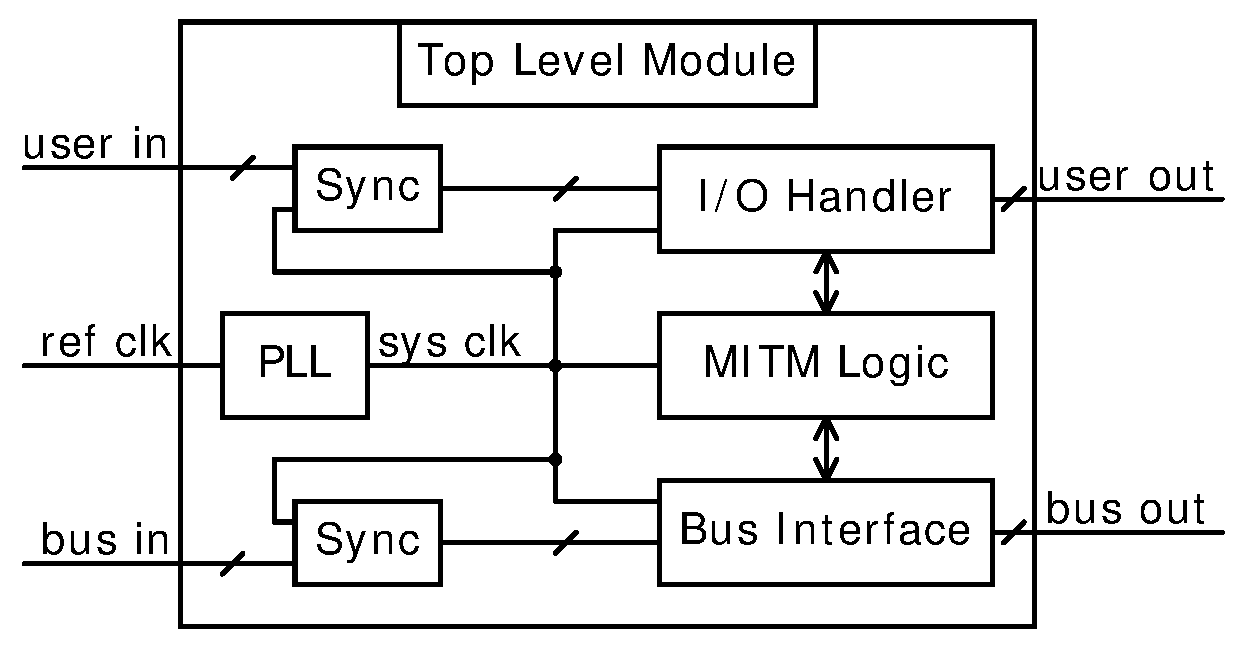
\includegraphics[width=0.8\textwidth]{images/topLevelModule.pdf}}
    \caption[Schéma hlavného modulu MITM obvodu]{Schéma hlavného modulu MITM obvodu.}
    \label{obr:topLevelModule}
\end{figure}

\section{Zbernicové rozhranie pre MITM logiku}
Najvýznamnejšou časťou našej implementácie je zbernicové rozhranie, pre MITM logiku, prostredníctvom ktorého možno vykonávať operácie nad komunikáciou. Cieľom rozhrania je zakryť detaily konkrétnej zbernice, ktorej protokol je fyzicky implementovaný na nižšej vrstve. Ako sme spomenuli v časti \ref{sek:masterSlave}, master-slave architektúru nie je možné na tejto úrovni abstrahovať, preto ju ponecháme na vyššiu vrstvu (MITM logika). Schéma, znázorňujúca princíp zapojenia zbernicového rozhrania je na obrázku \ref{obr:busInterface}.

\begin{figure}
    \centerline{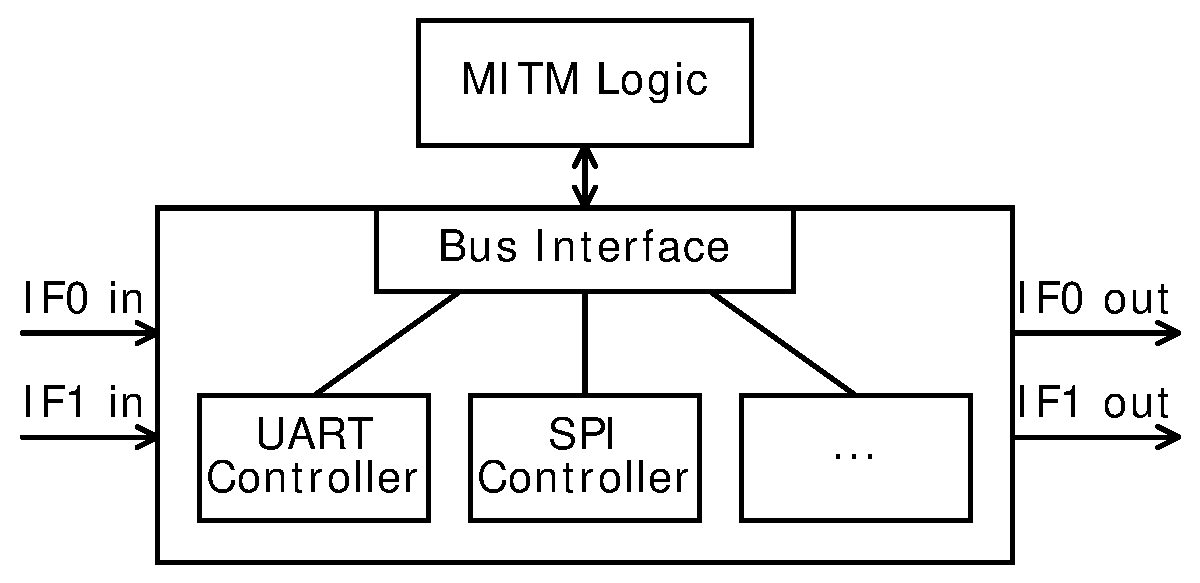
\includegraphics[width=0.8\textwidth]{images/busInterface.pdf}}
    \caption[Schéma zapojenia zbernicového rozhrania]{Schéma zapojenia zbernicového rozhrania. IF0 a IF1 predstavujú fyzické rozhrania k skutočným zariadeniam. Vstupné a výstupné linky pre jednotlivé rozhrania sa môžu líšiť v závislosti od konkrétnej zbernice a môžu byť asymetrické (master-slave architektúra).}
    \label{obr:busInterface}
\end{figure}

Cieľom rozhrania je abstrahovať najmä od fyzických vlastností ako napríklad spôsob kódovania logických hodnôt napätím, správna interpretácia prečítaných dát, vysielanie dát, generovanie hodinových signálov v prípade synchrónnej komunikácie a pod. Smerom k vyššej vrstve bude poskytovať rozhranie vstupy a výstupy pre vykonávanie MITM zásahov, prípadne pasívneho odpočúvania. Definícia vstupv a výstupov relevantných pre MITM logiku zbernicového rozhrania v jazyku Verilog je opísaná v algoritme \ref{alg:busInterface}.

Základnými sú vstupy a výstupy pre získanie dát prijatých na obidvoch fyzických rozhraniach zbernice a odvysielanie falošných dát na zvolenom rozhraní, prípadne oboch. Veľkosť (počet bitov) jedného bloku dát je možné nastaviť statickým parametrom. Pri niektorých zberniciach ako UART je táto veľkosť priamo určená parametrom protokolu, a treba ju príslušne nastaviť.

Ďalej poskytuje rozhranie možnosť prepínania medzi transparentným (forward) režimom a falošným (fake) režimom. Pri transparentnom režime je vysielanie falošných dát ignorované a zbernica fyzicky pripojí vstupy jednej strany na výstupy druhej strany. Tento mechanizmus je realizovaný pomocou multiplexora, ktorý opíšeme v časti \ref{subsek:multiplexor}. Vo falošnom režime rozhranie blokuje skutočnú komunikáciu a na výstupy pripojí falošné linky, po ktorých tečú falošné dáta, ktoré má pod kontrolou MITM logika. V prípade, že chceme komunikáciu iba blokovať, stačí zapnúť falošný režim a riadiaci vstup pre odvysielanie nastavených falošných dát ponecháme na logickej hodnote 0 (falošné dáta sa nikdy neodvysielajú).

Posledný mechanizmus, ktorý naše rozhranie umožňuje je tzv. keep-alive režim. Tento mechanizmus má význam pri zbernicových protokolov, ktoré na fyzickej vrstve používajú nejaký mechanizmus tzv. relácie, v rámci ktorej môže byť odvysielaných niekoľko blokov dát. Príkladom je zbernica SPI, pri ktorej môže master strana ponechať linku SS aktívnu po dlhšiu dobu a v rámci tohoto intervalu môže prebehnúť niekoľko výmen dátových blokov. V prípade, že režim keep-alive je zapnutý ponechá FPGA implementácia konkrétnej zbernice reláciu aktívnu a bude čakať na ďalšie inštrukcie z vyššej vrstvy. Napríklad v prípade SPI zbernice to znamená, že linka SS zostane aktívna aj po odvysielaní falošných dát a SPI implementácia bude čakať na riadiaci vstup pre odvysielanie ďalšieho bloku dát. Mechanizmus keep-alive nie je aplikovateľný na rozhraní, kde simulujeme slave stranu, nakoľko reláciu vždy riadi master.

Na slave strane je naopak potrebné zabezpečiť, aby sa falošné dáta odvysielali v správnom okamihu (komunikáciu riadi master). Pre tento účel využijeme binárny statusový výstup, ktorý indikuje, či je rozhranie na danej strane pripravené vysielať dáta. Implementácia rozhrania môže týmto výstupom signalizovať, že nie je pripravené odvysielať ďalšie dáta, napríklad z dôvodu, že aktuálne práve vysiela predošlé dáta. Implementácia rozhrania na slave strane zároveň bude signalizovať, že nie je pripravená odvysielať dáta aj v prípade, že to momentálne konkrétny master-slave protokol neumožňuje napriek tomu, že slave strana aktuálne nie je činná.

\begin{lstlisting}[float,language=Verilog,caption={Definícia vstupov a výstupov zbernicového rozhrania pre MITM logiku. Parameter NUM\_DATA\_BITS nastaví veľkosť bloku prijímaných/vysielaných dát.},label=alg:busInterface]
// riadiace vstupy
input wire fake_if0_select,     // zapne falošný mód na IF1->IF0
input wire fake_if1_select,     // zapne falošný mód na IF0->IF1
input wire fake_if0_send_start, // spustí vysielanie falošných dát
input wire fake_if1_send_start, // spustí vysielanie falošných dát
input wire fake_if0_keep_alive, // zapne keep-alive na IF0
input wire fake_if1_keep_alive, // zapne keep-alive na IF1

// statusové výstupy
output wire if0_recv_new_data,  // signalizuje prijatie nových dát
output wire if1_recv_new_data,  // signalizuje prijatie nových dát
output wire fake_if0_send_ready,// IF0 je pripravené vysielať   
output wire fake_if1_send_ready,// IF1 je pripravené vysielať   
output wire fake_if0_send_done,// signalizuje úspešné odvysielanie
output wire fake_if1_send_done,// signalizuje úspešné odvysielanie

// samotné vysielané/prijímané dáta
input wire [NUM_DATA_BITS-1:0] fake_if0_send_data, // falošné dáta
input wire [NUM_DATA_BITS-1:0] fake_if1_send_data, // falošné dáta
output wire [NUM_DATA_BITS-1:0] real_if0_recv_data,// skutočné dáta
output wire [NUM_DATA_BITS-1:0] real_if1_recv_data,// skutočné dáta
\end{lstlisting}

\section{Primitíva}

\subsection{Synchronizátor}\label{subsek:synchronizer}

\subsection{Detektor hrán}

\subsection{Výstupný multiplexor}\label{subsek:multiplexor}

\subsection{Sériový buffer pre čítanie a zápis}

\subsection{Čítač}

\subsection{Generátor impulzov}

\section{Vstup a výstup}

\section{Implementácia UART zbernice}

\section{Implementácia SPI zbernice}

\section{Vzorová implementácia MITM logiky}

\section{Konfigurácia, zapojenie a spustenie MITM obvodu}
Táto konfigurácia, ktorá definuje pripojenie fyzických I/O portov k zodpovedajúcim vstupom/výstupom hlavného modulu, je na úrovni zdrojového kóduv špecialnom súboreToto pripojenie je 